% !TEX root = review.tex

\subsection{Experimental methods}
\label{ssec:exp}

Two experimental methods are widely used in current high pressure research:
diamond anvil cell (DAC) and shock wave (SW).

DAC method is a static experimental method. The high pressure is produced by two beveled diamonds. \ce{Re} and stainless steel are used as gaskets, they are drilled holes before sample loading.
\ce{NaCl}, \ce{MgO}, and \ce{Al2O3} are served as pressure media and heating insulators in some experiments\cite{Anonymous:2004gu}.
\ce{Ar} gas or some other inert gases are often used to eliminate water
and oxygen, and also are pressure media.
High temperature can be produced by laser shone through diamonds.
The temperature is measured by pyrometric techniques,
and the melting of sample is observed by
visual inspection or X-ray spectroscopy\cite{Sola:2009dw}.

\begin{figure}[h]
	\centering
	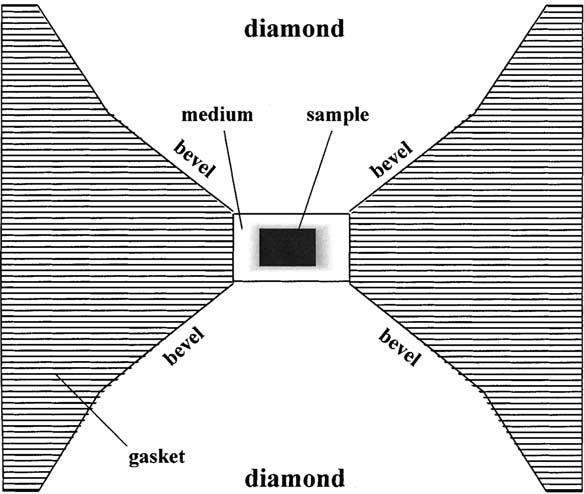
\includegraphics[width=0.5\linewidth]{DAC}
	\caption{Cross-section of a sample loaded in a diamond anvil cell with beveled diamonds. Note that the size of the gasket hole is the same as that of the diamond culet\cite{Anonymous:2004gu}.}
	\label{fig:dac}
\end{figure}

% Table generated by Excel2LaTeX from sheet 'Sheet1'
\begin{table}[htbp]
	\centering
	\caption{DAC experiments' conditions by years. If multiple pressures
		and temperatures were measured in experiments,
		only the highest is listed. Room temperature here is assumed to be
		\SI{298}{\kelvin} if not explicitly mentioned in the paper.}
	\begin{tabular}{ccc}
		\toprule
		year                              & $P$(\si{\giga\pascal}) & $T$(\si{\kelvin}) \\
		\midrule
		Mao 1967\cite{Mao:1967iz}         & $30$                   & $296$             \\
		Mao 1990\cite{Mao:1990ev}         & $ 300.6 $              & $ 298 $           \\
		Yoo 1995\cite{Yoo:1995kx}         & $130$                  & $3500$            \\
		Shen 1998\cite{Shen:1998bt}       & $ 84 $                 & $ 3500 $          \\
		Mao 1999\cite{Mao:1999fg}         & $ 211 $                & $ 298 $           \\
		Ma 2004\cite{Anonymous:2004gu}    & $ 161 $                & $ 3000 $          \\
		Dewaele 2006\cite{Dewaele:2006ha} & $ 205 $                & $ 298 $           \\
		Tateno 2010\cite{Tateno:2010io}   & $ 377 $                & $ 5700 $          \\
		\bottomrule
	\end{tabular}%
	\label{tab:dac}%
\end{table}%

The SW experiment, on the other hand,
is a dynamic method.
A high-speed impactor, with a velocity of the
order of \SIrange{5}{10}{\kilo\meter\per\second} is fired at the sample, and upon impact it generates high pressure and increases the temperature of the sample\cite{Sola:2009dw}.
Fast optics are used to follow the behavior of the SW which propagates inside the sample.
Due to the adiabatic heating of the sample, temperature obtained by SW should be higher than static conditions at room temperature.
Usually, temperature is not directly measured, but deduced by integrating the appropriate thermodynamic equation using estimates for the specific heat and the Grüneisen parameter.
The onset of melting is detected by a discontinuity in the speed of sound of the sample.


